\documentclass[conference]{IEEEtran}
\IEEEoverridecommandlockouts
% The preceding line is only needed to identify funding in the first footnote. If that is unneeded, please comment it out.
\usepackage{cite}
\usepackage{amsmath,amssymb,amsfonts}
\usepackage{algorithmic}
\usepackage{graphicx}
\usepackage{textcomp}
\usepackage{xcolor}
\def\BibTeX{{\rm B\kern-.05em{\sc i\kern-.025em b}\kern-.08em
    T\kern-.1667em\lower.7ex\hbox{E}\kern-.125emX}}
%%%%% NEW MATH DEFINITIONS %%%%%
\usepackage{bm}
% Mark sections of captions for referring to divisions of figures
\newcommand{\figleft}{{\em (Left)}}
\newcommand{\figcenter}{{\em (Center)}}
\newcommand{\figright}{{\em (Right)}}
\newcommand{\figtop}{{\em (Top)}}
\newcommand{\figbottom}{{\em (Bottom)}}
\newcommand{\captiona}{{\em (a)}}
\newcommand{\captionb}{{\em (b)}}
\newcommand{\captionc}{{\em (c)}}
\newcommand{\captiond}{{\em (d)}}

% Highlight a newly defined term
\newcommand{\newterm}[1]{{\bf #1}}


% Figure reference, lower-case.
\def\figref#1{figure~\ref{#1}}
% Figure reference, capital. For start of sentence
\def\Figref#1{Figure~\ref{#1}}
\def\twofigref#1#2{figures \ref{#1} and \ref{#2}}
\def\quadfigref#1#2#3#4{figures \ref{#1}, \ref{#2}, \ref{#3} and \ref{#4}}
% Section reference, lower-case.
\def\secref#1{section~\ref{#1}}
% Section reference, capital.
\def\Secref#1{Section~\ref{#1}}
% Reference to two sections.
\def\twosecrefs#1#2{sections \ref{#1} and \ref{#2}}
% Reference to three sections.
\def\secrefs#1#2#3{sections \ref{#1}, \ref{#2} and \ref{#3}}
% Reference to an equation, lower-case.
\def\eqref#1{equation~\ref{#1}}
% Reference to an equation, upper case
\def\Eqref#1{Equation~\ref{#1}}
% A raw reference to an equation---avoid using if possible
\def\plaineqref#1{\ref{#1}}
% Reference to a chapter, lower-case.
\def\chapref#1{chapter~\ref{#1}}
% Reference to an equation, upper case.
\def\Chapref#1{Chapter~\ref{#1}}
% Reference to a range of chapters
\def\rangechapref#1#2{chapters\ref{#1}--\ref{#2}}
% Reference to an algorithm, lower-case.
\def\algref#1{algorithm~\ref{#1}}
% Reference to an algorithm, upper case.
\def\Algref#1{Algorithm~\ref{#1}}
\def\twoalgref#1#2{algorithms \ref{#1} and \ref{#2}}
\def\Twoalgref#1#2{Algorithms \ref{#1} and \ref{#2}}
% Reference to a part, lower case
\def\partref#1{part~\ref{#1}}
% Reference to a part, upper case
\def\Partref#1{Part~\ref{#1}}
\def\twopartref#1#2{parts \ref{#1} and \ref{#2}}

\def\ceil#1{\lceil #1 \rceil}
\def\floor#1{\lfloor #1 \rfloor}
\def\1{\bm{1}}
\newcommand{\train}{\mathcal{D}}
\newcommand{\valid}{\mathcal{D_{\mathrm{valid}}}}
\newcommand{\test}{\mathcal{D_{\mathrm{test}}}}

\def\eps{{\epsilon}}


% Random variables
\def\reta{{\textnormal{$\eta$}}}
\def\ra{{\textnormal{a}}}
\def\rb{{\textnormal{b}}}
\def\rc{{\textnormal{c}}}
\def\rd{{\textnormal{d}}}
\def\re{{\textnormal{e}}}
\def\rf{{\textnormal{f}}}
\def\rg{{\textnormal{g}}}
\def\rh{{\textnormal{h}}}
\def\ri{{\textnormal{i}}}
\def\rj{{\textnormal{j}}}
\def\rk{{\textnormal{k}}}
\def\rl{{\textnormal{l}}}
% rm is already a command, just don't name any random variables m
\def\rn{{\textnormal{n}}}
\def\ro{{\textnormal{o}}}
\def\rp{{\textnormal{p}}}
\def\rq{{\textnormal{q}}}
\def\rr{{\textnormal{r}}}
\def\rs{{\textnormal{s}}}
\def\rt{{\textnormal{t}}}
\def\ru{{\textnormal{u}}}
\def\rv{{\textnormal{v}}}
\def\rw{{\textnormal{w}}}
\def\rx{{\textnormal{x}}}
\def\ry{{\textnormal{y}}}
\def\rz{{\textnormal{z}}}

% Random vectors
\def\rvepsilon{{\mathbf{\epsilon}}}
\def\rvtheta{{\mathbf{\theta}}}
\def\rva{{\mathbf{a}}}
\def\rvb{{\mathbf{b}}}
\def\rvc{{\mathbf{c}}}
\def\rvd{{\mathbf{d}}}
\def\rve{{\mathbf{e}}}
\def\rvf{{\mathbf{f}}}
\def\rvg{{\mathbf{g}}}
\def\rvh{{\mathbf{h}}}
\def\rvu{{\mathbf{i}}}
\def\rvj{{\mathbf{j}}}
\def\rvk{{\mathbf{k}}}
\def\rvl{{\mathbf{l}}}
\def\rvm{{\mathbf{m}}}
\def\rvn{{\mathbf{n}}}
\def\rvo{{\mathbf{o}}}
\def\rvp{{\mathbf{p}}}
\def\rvq{{\mathbf{q}}}
\def\rvr{{\mathbf{r}}}
\def\rvs{{\mathbf{s}}}
\def\rvt{{\mathbf{t}}}
\def\rvu{{\mathbf{u}}}
\def\rvv{{\mathbf{v}}}
\def\rvw{{\mathbf{w}}}
\def\rvx{{\mathbf{x}}}
\def\rvy{{\mathbf{y}}}
\def\rvz{{\mathbf{z}}}

% Elements of random vectors
\def\erva{{\textnormal{a}}}
\def\ervb{{\textnormal{b}}}
\def\ervc{{\textnormal{c}}}
\def\ervd{{\textnormal{d}}}
\def\erve{{\textnormal{e}}}
\def\ervf{{\textnormal{f}}}
\def\ervg{{\textnormal{g}}}
\def\ervh{{\textnormal{h}}}
\def\ervi{{\textnormal{i}}}
\def\ervj{{\textnormal{j}}}
\def\ervk{{\textnormal{k}}}
\def\ervl{{\textnormal{l}}}
\def\ervm{{\textnormal{m}}}
\def\ervn{{\textnormal{n}}}
\def\ervo{{\textnormal{o}}}
\def\ervp{{\textnormal{p}}}
\def\ervq{{\textnormal{q}}}
\def\ervr{{\textnormal{r}}}
\def\ervs{{\textnormal{s}}}
\def\ervt{{\textnormal{t}}}
\def\ervu{{\textnormal{u}}}
\def\ervv{{\textnormal{v}}}
\def\ervw{{\textnormal{w}}}
\def\ervx{{\textnormal{x}}}
\def\ervy{{\textnormal{y}}}
\def\ervz{{\textnormal{z}}}

% Random matrices
\def\rmA{{\mathbf{A}}}
\def\rmB{{\mathbf{B}}}
\def\rmC{{\mathbf{C}}}
\def\rmD{{\mathbf{D}}}
\def\rmE{{\mathbf{E}}}
\def\rmF{{\mathbf{F}}}
\def\rmG{{\mathbf{G}}}
\def\rmH{{\mathbf{H}}}
\def\rmI{{\mathbf{I}}}
\def\rmJ{{\mathbf{J}}}
\def\rmK{{\mathbf{K}}}
\def\rmL{{\mathbf{L}}}
\def\rmM{{\mathbf{M}}}
\def\rmN{{\mathbf{N}}}
\def\rmO{{\mathbf{O}}}
\def\rmP{{\mathbf{P}}}
\def\rmQ{{\mathbf{Q}}}
\def\rmR{{\mathbf{R}}}
\def\rmS{{\mathbf{S}}}
\def\rmT{{\mathbf{T}}}
\def\rmU{{\mathbf{U}}}
\def\rmV{{\mathbf{V}}}
\def\rmW{{\mathbf{W}}}
\def\rmX{{\mathbf{X}}}
\def\rmY{{\mathbf{Y}}}
\def\rmZ{{\mathbf{Z}}}

% Elements of random matrices
\def\ermA{{\textnormal{A}}}
\def\ermB{{\textnormal{B}}}
\def\ermC{{\textnormal{C}}}
\def\ermD{{\textnormal{D}}}
\def\ermE{{\textnormal{E}}}
\def\ermF{{\textnormal{F}}}
\def\ermG{{\textnormal{G}}}
\def\ermH{{\textnormal{H}}}
\def\ermI{{\textnormal{I}}}
\def\ermJ{{\textnormal{J}}}
\def\ermK{{\textnormal{K}}}
\def\ermL{{\textnormal{L}}}
\def\ermM{{\textnormal{M}}}
\def\ermN{{\textnormal{N}}}
\def\ermO{{\textnormal{O}}}
\def\ermP{{\textnormal{P}}}
\def\ermQ{{\textnormal{Q}}}
\def\ermR{{\textnormal{R}}}
\def\ermS{{\textnormal{S}}}
\def\ermT{{\textnormal{T}}}
\def\ermU{{\textnormal{U}}}
\def\ermV{{\textnormal{V}}}
\def\ermW{{\textnormal{W}}}
\def\ermX{{\textnormal{X}}}
\def\ermY{{\textnormal{Y}}}
\def\ermZ{{\textnormal{Z}}}

% Vectors
\def\vzero{{\bm{0}}}
\def\vone{{\bm{1}}}
\def\vmu{{\bm{\mu}}}
\def\vtheta{{\bm{\theta}}}
\def\va{a}
\def\vb{{\bm{b}}}
\def\vc{{\bm{c}}}
\def\vd{{\bm{d}}}
\def\ve{{\bm{e}}}
\def\vf{{\bm{f}}}
\def\vg{{\bm{g}}}
\def\vh{{\bm{h}}}
\def\vi{{\bm{i}}}
\def\vj{{\bm{j}}}
\def\vk{{\bm{k}}}
\def\vl{{\bm{l}}}
\def\vm{{\bm{m}}}
\def\vn{{\bm{n}}}
\def\vo{{\bm{o}}}
\def\vp{{\bm{p}}}
\def\vq{{\bm{q}}}
\def\vr{{\bm{r}}}
\def\vs{{\bm{s}}}
\def\vt{{\bm{t}}}
\def\vu{{\bm{u}}}
\def\vv{{\bm{v}}}
\def\vw{{\bm{w}}}
\def\vx{{\bm{x}}}
\def\vy{{\bm{y}}}
\def\vz{{\bm{z}}}

% Elements of vectors
\def\evalpha{{\alpha}}
\def\evbeta{{\beta}}
\def\evepsilon{{\epsilon}}
\def\evlambda{{\lambda}}
\def\evomega{{\omega}}
\def\evmu{{\mu}}
\def\evpsi{{\psi}}
\def\evsigma{{\sigma}}
\def\evtheta{{\theta}}
\def\eva{{a}}
\def\evb{{b}}
\def\evc{{c}}
\def\evd{{d}}
\def\eve{{e}}
\def\evf{{f}}
\def\evg{{g}}
\def\evh{{h}}
\def\evi{{i}}
\def\evj{{j}}
\def\evk{{k}}
\def\evl{{l}}
\def\evm{{m}}
\def\evn{{n}}
\def\evo{{o}}
\def\evp{{p}}
\def\evq{{q}}
\def\evr{{r}}
\def\evs{{s}}
\def\evt{{t}}
\def\evu{{u}}
\def\evv{{v}}
\def\evw{{w}}
\def\evx{{x}}
\def\evy{{y}}
\def\evz{{z}}

% Matrix
\def\mA{{\bm{A}}}
\def\mB{{\bm{B}}}
\def\mC{{\bm{C}}}
\def\mD{{\bm{D}}}
\def\mE{{\bm{E}}}
\def\mF{{\bm{F}}}
\def\mG{{\bm{G}}}
\def\mH{{\bm{H}}}
\def\mI{{\bm{I}}}
\def\mJ{{\bm{J}}}
\def\mK{{\bm{K}}}
\def\mL{{\bm{L}}}
\def\mM{{\bm{M}}}
\def\mN{{\bm{N}}}
\def\mO{{\bm{O}}}
\def\mP{{\bm{P}}}
\def\mQ{{\bm{Q}}}
\def\mR{{\bm{R}}}
\def\mS{{\bm{S}}}
\def\mT{{\bm{T}}}
\def\mU{{\bm{U}}}
\def\mV{{\bm{V}}}
\def\mW{{\bm{W}}}
\def\mX{{\bm{X}}}
\def\mY{{\bm{Y}}}
\def\mZ{{\bm{Z}}}
\def\mBeta{{\bm{\beta}}}
\def\mPhi{{\bm{\Phi}}}
\def\mLambda{{\bm{\Lambda}}}
\def\mSigma{{\bm{\Sigma}}}

% Tensor
\DeclareMathAlphabet{\mathsfit}{\encodingdefault}{\sfdefault}{m}{sl}
\SetMathAlphabet{\mathsfit}{bold}{\encodingdefault}{\sfdefault}{bx}{n}
\newcommand{\tens}[1]{\bm{\mathsfit{#1}}}
\def\tA{{\tens{A}}}
\def\tB{{\tens{B}}}
\def\tC{{\tens{C}}}
\def\tD{{\tens{D}}}
\def\tE{{\tens{E}}}
\def\tF{{\tens{F}}}
\def\tG{{\tens{G}}}
\def\tH{{\tens{H}}}
\def\tI{{\tens{I}}}
\def\tJ{{\tens{J}}}
\def\tK{{\tens{K}}}
\def\tL{{\tens{L}}}
\def\tM{{\tens{M}}}
\def\tN{{\tens{N}}}
\def\tO{{\tens{O}}}
\def\tP{{\tens{P}}}
\def\tQ{{\tens{Q}}}
\def\tR{{\tens{R}}}
\def\tS{{\tens{S}}}
\def\tT{{\tens{T}}}
\def\tU{{\tens{U}}}
\def\tV{{\tens{V}}}
\def\tW{{\tens{W}}}
\def\tX{{\tens{X}}}
\def\tY{{\tens{Y}}}
\def\tZ{{\tens{Z}}}


% Graph
\def\gA{{\mathcal{A}}}
\def\gB{{\mathcal{B}}}
\def\gC{{\mathcal{C}}}
\def\gD{{\mathcal{D}}}
\def\gE{{\mathcal{E}}}
\def\gF{{\mathcal{F}}}
\def\gG{{\mathcal{G}}}
\def\gH{{\mathcal{H}}}
\def\gI{{\mathcal{I}}}
\def\gJ{{\mathcal{J}}}
\def\gK{{\mathcal{K}}}
\def\gL{{\mathcal{L}}}
\def\gM{{\mathcal{M}}}
\def\gN{{\mathcal{N}}}
\def\gO{{\mathcal{O}}}
\def\gP{{\mathcal{P}}}
\def\gQ{{\mathcal{Q}}}
\def\gR{{\mathcal{R}}}
\def\gS{{\mathcal{S}}}
\def\gT{{\mathcal{T}}}
\def\gU{{\mathcal{U}}}
\def\gV{{\mathcal{V}}}
\def\gW{{\mathcal{W}}}
\def\gX{{\mathcal{X}}}
\def\gY{{\mathcal{Y}}}
\def\gZ{{\mathcal{Z}}}

% Sets
\def\sA{{\mathbb{A}}}
\def\sB{{\mathbb{B}}}
\def\sC{{\mathbb{C}}}
\def\sD{{\mathbb{D}}}
% Don't use a set called E, because this would be the same as our symbol
% for expectation.
\def\sF{{\mathbb{F}}}
\def\sG{{\mathbb{G}}}
\def\sH{{\mathbb{H}}}
\def\sI{{\mathbb{I}}}
\def\sJ{{\mathbb{J}}}
\def\sK{{\mathbb{K}}}
\def\sL{{\mathbb{L}}}
\def\sM{{\mathbb{M}}}
\def\sN{{\mathbb{N}}}
\def\sO{{\mathbb{O}}}
\def\sP{{\mathbb{P}}}
\def\sQ{{\mathbb{Q}}}
\def\sR{{\mathbb{R}}}
\def\sS{{\mathbb{S}}}
\def\sT{{\mathbb{T}}}
\def\sU{{\mathbb{U}}}
\def\sV{{\mathbb{V}}}
\def\sW{{\mathbb{W}}}
\def\sX{{\mathbb{X}}}
\def\sY{{\mathbb{Y}}}
\def\sZ{{\mathbb{Z}}}

% Entries of a matrix
\def\emLambda{{\Lambda}}
\def\emA{{A}}
\def\emB{{B}}
\def\emC{{C}}
\def\emD{{D}}
\def\emE{{E}}
\def\emF{{F}}
\def\emG{{G}}
\def\emH{{H}}
\def\emI{{I}}
\def\emJ{{J}}
\def\emK{{K}}
\def\emL{{L}}
\def\emM{{M}}
\def\emN{{N}}
\def\emO{{O}}
\def\emP{{P}}
\def\emQ{{Q}}
\def\emR{{R}}
\def\emS{{S}}
\def\emT{{T}}
\def\emU{{U}}
\def\emV{{V}}
\def\emW{{W}}
\def\emX{{X}}
\def\emY{{Y}}
\def\emZ{{Z}}
\def\emSigma{{\Sigma}}

% entries of a tensor
% Same font as tensor, without \bm wrapper
\newcommand{\etens}[1]{\mathsfit{#1}}
\def\etLambda{{\etens{\Lambda}}}
\def\etA{{\etens{A}}}
\def\etB{{\etens{B}}}
\def\etC{{\etens{C}}}
\def\etD{{\etens{D}}}
\def\etE{{\etens{E}}}
\def\etF{{\etens{F}}}
\def\etG{{\etens{G}}}
\def\etH{{\etens{H}}}
\def\etI{{\etens{I}}}
\def\etJ{{\etens{J}}}
\def\etK{{\etens{K}}}
\def\etL{{\etens{L}}}
\def\etM{{\etens{M}}}
\def\etN{{\etens{N}}}
\def\etO{{\etens{O}}}
\def\etP{{\etens{P}}}
\def\etQ{{\etens{Q}}}
\def\etR{{\etens{R}}}
\def\etS{{\etens{S}}}
\def\etT{{\etens{T}}}
\def\etU{{\etens{U}}}
\def\etV{{\etens{V}}}
\def\etW{{\etens{W}}}
\def\etX{{\etens{X}}}
\def\etY{{\etens{Y}}}
\def\etZ{{\etens{Z}}}

% The true underlying data generating distribution
\newcommand{\pdata}{p_{\rm{data}}}
% The empirical distribution defined by the training set
\newcommand{\ptrain}{\hat{p}_{\rm{data}}}
\newcommand{\Ptrain}{\hat{P}_{\rm{data}}}
% The model distribution
\newcommand{\pmodel}{p_{\rm{model}}}
\newcommand{\Pmodel}{P_{\rm{model}}}
\newcommand{\ptildemodel}{\tilde{p}_{\rm{model}}}
% Stochastic autoencoder distributions
\newcommand{\pencode}{p_{\rm{encoder}}}
\newcommand{\pdecode}{p_{\rm{decoder}}}
\newcommand{\precons}{p_{\rm{reconstruct}}}

\newcommand{\laplace}{\mathrm{Laplace}} % Laplace distribution

\newcommand{\E}{\mathbb{E}}
\newcommand{\Ls}{\mathcal{L}}
\newcommand{\R}{\mathbb{R}}
\newcommand{\emp}{\tilde{p}}
\newcommand{\lr}{\alpha}
\newcommand{\reg}{\lambda}
\newcommand{\rect}{\mathrm{rectifier}}
\newcommand{\softmax}{\mathrm{softmax}}
\newcommand{\sigmoid}{\sigma}
\newcommand{\softplus}{\zeta}
\newcommand{\KL}{D_{\mathrm{KL}}}
\newcommand{\Var}{\mathrm{Var}}
\newcommand{\standarderror}{\mathrm{SE}}
\newcommand{\Cov}{\mathrm{Cov}}
% Wolfram Mathworld says $L^2$ is for function spaces and $\ell^2$ is for vectors
% But then they seem to use $L^2$ for vectors throughout the site, and so does
% wikipedia.
\newcommand{\normlzero}{L^0}
\newcommand{\normlone}{L^1}
\newcommand{\normltwo}{L^2}
\newcommand{\normlp}{L^p}
\newcommand{\normmax}{L^\infty}

\newcommand{\parents}{Pa} % See usage in notation.tex. Chosen to match Daphne's book.


\def\ContentSet{{\sC}}
\def\OwnerSet{{\sO}}
\def\content{{c}}
\def\owner{{o}}
\def\simfunc{{s}}
\def\threshold{{\lambda}}
\begin{document}

\title{Proof of Novelty\\
\thanks{This short paper was written for the VIRTUAL DESIGN CHALLENGE FOR AUTHENTICATING AND PROTECTING FULL MOTION VIDEOS: https://blockchain.ubc.ca/news/virtual-design-challenge-authenticating-and-protecting-full-motion-videos}}

\author{\IEEEauthorblockN{Daniel Severo}
\IEEEauthorblockA{
\textit{Independent Scientist}\\
S\~{a}o Paulo, Brazil\\ 
danielsouzasevero@gmail.com}}

\maketitle
\begin{abstract}
We propose a design for securing novelty of archived content in distributed ledgers, called \emph{Proof of Novelty}. What constitutes as novel is decided through a consensus mechanism together with a similarity function, which is selected according to the content type (e.g. full-motion videos, textual documents). Scalability is guaranteed by forming a validation committee with cryptographic sortition, which use statistical hypothesis testing to decide on the probability of a content being novel or not. The system can trade-off computational with statistical performance by manipulating parameters. We discuss the usage of this design to secure the novelty of full-motion videos and end with a proposal of future lines of research that can extend the systems capabilities.
% UNTITLED is a Distributed Patent System design proposal equipped with a Prior Art search mechanism. Patentability requirements are defined through a consensus protocol using Smart Contracts and collaborative training of machine learning algorithms. Removing the patent clerk and shifting the burden of proof of patentability to the patentee, we guarantee scalability and efficiency of the blockchain. The system is highly sensitive to the invention’s medium (e.g. audio files, textual documents) as it defines the class of algorithms employed to calculate similarity, which in turn defines what constitutes as prior art. We show how UNTITLED can be applied to full-motion video archives to protect against tampering and dissemination of false information through Deepfakes.
\end{abstract}

\begin{IEEEkeywords}
blockchain, patent, smart contracts, prior art, full-motion videos, proof of novelty
\end{IEEEkeywords}

\section{Introduction}
Guaranteeing novelty and authenticity of modern media content (e.g. full-motion videos, textual documents, audio files) is crucial for decision making in areas such as court trials and journalism. Failing to do so risks undermining the credibility of the decision maker. For example, journalists fact check their findings before publishing news articles \cite{graves2016deciding}; patent clerks exhaustively gather evidence of absence of prior art before emitting patent certificates \cite{callaert2006traces}; and media archives (e.g. YouTube) protect artists by taking down copyright-infringing content \cite{o2006digital}. Scholarly peer review systems also share this characteristic, where a reviewer is tasked with evaluating the claims made in an academic paper during the process of submission to a conference or journal.

The central concepts underlying the aforementioned examples are \emph{novelty} and \emph{authenticity}. An item is deemed authentic when its provenance is indisputable. What constitutes as novel is often the cause of discourse due to its subjective nature and the trust bestowed upon a centralized agent to discriminate on what is, and what is is not, genuinely novel. More recently, a new issue has emerged due to the proliferation of digital content in the internet age; verifying novelty against large archives. Even if the definition of novelty can be agreed upon by interested parties, exhaustively comparing candidate and existing contents can be computationally intractable due to large data volumes (e.g. 500 hours of video images are uploaded to YouTube every minute \cite{robertson2015500}). Defining and securing authenticity is comparably more mature and has benefited considerably in recent years with the advent of Digital Signatures \cite{pointcheval2000security}.

In the case of media archives, checking for novelty prior to acceptance can be seen as a way of preserving the moral integrity of \emph{currently} archived content. A malicious agent can attack content by submitting a modified version and leverage social media as a vector for propagating false information. Considerable time may pass until the false content is debunked and may cause irreversible damage to the owner of the original content. Complexity of attacks range from audio manipulation and video context clipping to modern computer vision techniques (e.g. Deepfakes) \cite{chesney2018deep}. 

Pior work has tackled the issue of detecting video tampering \emph{from within} the archive by using content-sensitive identifiers (e.g. digests from cryptographic hash functions) at the moment of content ingestion and storing them in permanent ledgers (e.g. blockchains). The same techniques are also employed for combating spoofing, where content provenance is contested; closely relating to issues with authenticity \cite{hasan2019combating}. To the best of our knowledge, little to no work has been done in preventing the ill-usage of created content.

In this paper, we contribute with

\begin{enumerate}
    \item a consensus mechanism for securing genuity, called \emph{Proof of Novelty}\footnote{https://github.com/dsevero/Proof-of-Novelty} (PoN);
    \item an approach to combat false media content in digital archives with PoN.
\end{enumerate}

Our design draws inspiration from \emph{Patent Systems}. We discuss shortcomings of our approach as well as model details in the following sections.

\section{Background}
\subsection{Patent Systems and Prior Art}
A patent is a legal document that provides proof of ownership of intellectual property (IP) \cite{callaert2006traces}. It is commonly issued by government run agencies to individuals or organizations. Its main function is to secure legal exclusivity regarding sales, production and distribution of the IP to the owner. The procedure of emission is initiated with a formal request by the party interested in obtaining the patent, called a \emph{patentee}. A \emph{patent clerk}, representing the emitting agency, is then attributed with the task of verifying patentability conditions such as (but not limited to) novelty and non-obviousness of the invention. This is done by collecting evidence of absence of previous similar work, called \emph{Prior Art}. Searching is done against niche databases specialized in storing technical documents \cite{callaert2006traces}.

Granting a patent is an attestation of novelty, conditioned on trust in the emitting agency. An improper Prior Art search can lead to erroneous conclusions of novelty regarding the patentee's invention \cite{bashir2010improving}. 

\subsection{Similarity Measures}
A similarity measure is any function that quantifies the degree of similarity between objects \cite{lesot2009similarity}. For example, the Jaccard index measures similarity between sets $\sA$ and $\sB$, by comparing the number of common elements. Formally, it is the ratio between the the intersection and union, and varies between 0 and 1; $J(\sA, \sB) = \vert\sA\cap\sB\vert/\vert\sA\cup\sB\vert$. These metrics are common in applications regarding information retrieval (e.g. search systems) and recommendation systems \cite{metzler2007similarity}.

Distance functions $d$ are common throughout literature and can be converted into a similarity measure by a simple transformation such as $d \to \frac{1}{1+d}$. Both distance and similarity measures are sensitive to their domain. For example, the Jaccard index previously mentioned can not be used directly on real valued data (what would $J(5, 2.4)$ mean?)  \cite{lesot2009similarity}.

There is a vast amount of literature addressing metrics for text, full-motion videos and audio applications \cite{kulis2013metric}. The field of \emph{Similarity Learning} is concerned with the task of learning similarity and distance functions through the usage of labeled examples and Machine Learning techniques (i.e. Supervised Machine Learning) \cite{kulis2013metric}.
 

\subsection{Blockchains}
A Blockchain is a growing list of ordered records that contain digitally signed transactions \cite{antonopoulos2018mastering}. Appending a record to the chain is done by cryptographically hashing the list and adding it to the incoming record. Blockchains are considered immutable, since altering a transaction anywhere in the list would require recomputing the hash of all records that came after it \cite{antonopoulos2018mastering}. This data structure often lives on a distributed public peer-to-peer network, where all peers hold a copy of the list and must reach consensus on which incoming blocks should be appended. 

Multiple consensus mechanism have been proposed throughout literature. Examples are Proof of Work \cite{dwork1992pricing}, Stake \cite{king2012ppcoin} and Authority \cite{de2018pbft} (PoW, PoS, and PoA; respectively). Some protocols require partial centralization to be secure, such as PoS and PoA. PoW can be fully distributed, but is inefficient in the time it takes to append a new block to the chain and requires a surplus amount of resources \cite{dwork1992pricing}.

A \emph{Smart Contract} usually refers to a computer program that is executed collaboratively on a blockchain \cite{szabo1997idea}. Consensus on the state of execution of the program is reached through the consensus mechanisms previously mentioned. The name comes from its usage in enforcing terms of agreements between parties in a way that doesn't require trust in a centralized moderator, such as a government agency.

The \emph{Ethereum Virtual Machine} is a distributed blockchain system that implements a set of machine-level instructions similar to a general purpose computer \cite{wood2014ethereum}. It supports Smart Contracts, which are usually written in languages such as Solidity, Vyper and LLL. Programs running on the EVM can be used as the back-end (i.e. server-side) for software applications called \emph{Decentralized Apps} (Dapps).

\subsection{Cryptographic Sortition}
Sortition is the act of randomly selecting elements of a group to form a committee. It is usually associated with political systems as an alternative to elections, where representatives are selected by sampling from the population of eligible citizens. For element $i$, the probability $p_i$ of being selected is proportional to some non-negative real valued weight $\omega_i$, such as $p_i = \omega_i/\sum_i\omega_i$. Choosing equal weights (i.e. $\omega_i = \omega_j; \forall i,j$) results in a uniform distribution, where every element has the same chance of being selected.

Sortition can be used to scale blockchain systems, by forming a committee of peers to reach consensus on new blocks; possibly replacing PoW \cite{gilad2017algorand}. Although promising, a naive implementation can cause security concerns due to interactions between committee members and their exposure to malicious agents. Algorand \cite{gilad2017algorand} created a consensus protocol which forms committees without the need of interactions or exposure, using \emph{Cryptographic Sortition}. Any peer holding a private key can verify and prove self-membership in the committee using a \emph{Verifiable Random Function} \cite{micali1999verifiable}.

\subsection{Content-Addressable Storage}
Location-addressable systems reference resources based on location. Examples are everyday systems such as bank accounts, housing addresses, traditional databases, and the internet. Content-addressable systems use the content itself (usually in the form of a hash) as a locator \cite{atkin2010system}.

The \emph{InterPlanetary File System} (IPFS) \cite{benet2014ipfs} is a distributed content-addressable storage system that is commonly used with blockchain technology and Smart Contracts. Referencing stored content by its cryptographic hash allows IPFS to remove duplicated files, as any two files that are exactly the same will have equal hashes.
\section{Problem Statement}
Let $\ContentSet$ represent a collection of content archived in a distributed content-addressable storage system such as IPFS. For each content $\content \in \ContentSet$ there exists some owner $\owner \in \OwnerSet$ such that the mapping $\content \to \owner$ is one-to-one but the inverse $\owner \to \content$ is one-to-many. In other words, one owner can have multiple contents, but each content has a unique owner. 

A \emph{similarity measure} on $\ContentSet$ is a function $\simfunc \colon \ContentSet^2 \to \mathbb{R}$ that takes a pair of contents as input and returns a scalar that captures the notion of what constitutes as similar. $s$ can be anything from an Artificial Neural Network to a simple comparison of descriptive statistics.

The system will accept or reject the insertion of a candidate $\content^\prime \notin \ContentSet$ based on a subset of similar content $$\sS(\content^\prime, \sV) = \left\{ \simfunc(\content,\content^\prime) \mid \forall \content \in \sV \subseteq \ContentSet \right\}$$

with some rule $\mathcal{H}$ 

$$\sS(\content^\prime, \sV) \xrightarrow{\mathcal{H}} r \in \text{\{accept, reject\}}$$

where $(\mathcal{H}, s)$ is defined through consensus.

Accepting $\content^\prime$ can be viewed as the equivalent of emitting a \emph{certificate of novelty}. The objective is to minimize the rate of false positives while maintaining a reasonable rate of acceptance. An owner $\owner$ wishing to prove novelty of $\content$ can do so by showing that $\content \in \ContentSet$ and $\content \xrightarrow{} \owner$ to any entity that trusts the system $\left(\mathcal{H}, \simfunc \right)$.

\section{Related Work}
Previous work has tackled the problem of authenticity (i.e. proving provenance) by securing files on content-addressable storage (e.g. IPFS) with blockchain technology. \cite{hasan2019combating} implements a Smart Contract on EVM where artists can register their content hosted on IPFS to be shared, modified, and purchased. The blockchain tracks a history of interactions and creates a hierarchy of parent-child relationships that makes it possible to trace content provenance. Bernstein \cite{Bernstein} is a decentralized app that implements a Patent System. It can prove ownership, existence and integrity (i.e. tamper-proof) of stored files. ARCHANGEL \cite{bui2019archangel} is a tamper-proof video archive equipped with a content hashing mechanism insensitive to most lossy compression algorithms.

None of these are capable of verifying novelty of files submitted to the system. A malicious agent can download content, modify it for ill-usage, and submit it back to the blockchain. Even though it is possible to prove that the modified content was inserted after the original (since blockchains are ordered lists), there is still the issue of locating the original content for comparison. 

MediaChain was a peer-to-peer database for users to collaborate on open-media. It contained a metadata resolution protocol that was intended to map similar content to the same metadata. The project was halted when bought by Spotify in 2017 and the solver was never fully implemented \cite{perez2017spotify}.



% TODO \\
% - ARCHANGEL: TCH needs overfitting; doesn't address discovery\\
% - Mediachain\\
% - Locality-sensitive hashing\\
% - https://arxiv.org/abs/1901.03136\\
\section{Design Proposal}
An overview of the system is presented through narrative. Details are addressed in later subsections. 

\begin{figure}
    \centering
    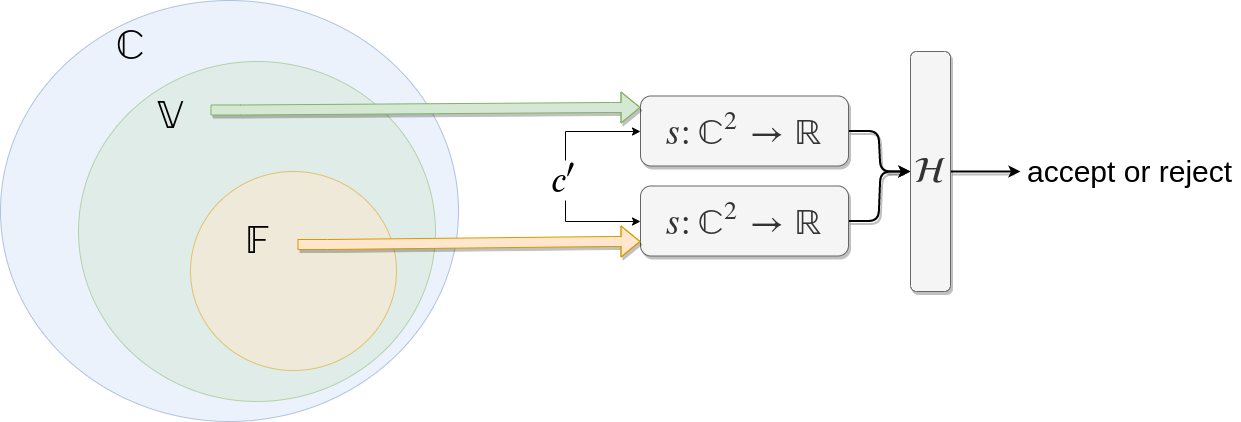
\includegraphics[width=0.45\textwidth, keepaspectratio]{assets/pon-diagram-full-icbc2020.png}
    \caption{System overview. The set $\ContentSet$ represents the content archive; $\sV$ is a subset of $\ContentSet$ and is created by the blockchain to be validated by the owner of $\content$; $\sF$ is chosen with cryptographic sortition as a random subset of $\sV$ and is used a sample for validation; $\simfunc$ is a similarity function and $\mathcal{H}$ is the rule (most likely a hypothesis test) that accepts or rejects $\content$.}
    \label{fig:diagram}
\end{figure}

\subsection{Overview}\label{overview}
Consider a credible archive $\ContentSet$ of similar content, with content-addressable hashes secured on a smart contract enabled blockchain, an associated similarity measure $\simfunc$, and an acceptance/rejection rule $\mathcal{H}$. For example, arXiv articles stored on IPFS with community defined $s$ and $\mathcal{H}$ secured by Ethereum. Note that credibility is a consensus amongst peers and not an intrinsic property of the archive (e.g. scholarly peer-reviewed venues). An owner $\owner^\prime$,  wishing to prove novelty of content $\content^\prime \notin \ContentSet$, makes a transaction on the blockchain and receives a random subset of content-hashes of elements $\content \in \sV \subseteq \ContentSet$. The owner now uses $\simfunc$ to calculate the similarity of $\content^\prime$ with the elements of $\sV$ (i.e. $\sS(\content^\prime, \sV)$) and submits the calculations back to the smart contract for evaluation. Using cryptographic sortition, the smart contract chooses a random committee that is tasked with off-chain verification of a subset of the results, $\sS(\content^\prime, \sF \subseteq \sV)$. Consensus is reached by the committee regarding the legitimacy of $\sS(\content^\prime, \sV)$, and $\content^\prime$ is accepted or rejected into the archive based on the rule $\mathcal{H}$.

\subsection{Choosing $\sV$ and $\sF$}
The degree of novelty verified by the system is directly related to the cardinality (i.e. number of elements) of $\sV$, represented by $\vert\sV\vert$. Making $\sV = \ContentSet$ will guarantee that all files in the archive are compared against the candidate content $\content^\prime$, but will make the computation of $\sS(\content^\prime, \sV)$ resource intensive. Similarly, raising $\vert\sF\vert$ decreases the probability that an owner can successfully manipulate the values of $\sS(\content^\prime, \sV)$, but requires more computational power during the verification process by network peers.

Scalability of this solution comes from the fact that $\vert\sF\vert < \vert\sV\vert$, which is possible only if $\sF$ is hidden from the owner $\owner^\prime$. This means that the candidate does not know which values of $\sV$ will be verified by his peers, forcing him to compute $\simfunc(\content,\content^\prime)$ for all values of $\content \in \sV$. The probability of randomly guessing which elements are in $\sF$ can be made as low as required.

\subsection{Consensus of Peers Regarding $\sS(\content^\prime, \sV)$}
Using only $\sS(\content^\prime, \sF \subseteq \sV)$, the committee must infer if $\sS(\content^\prime, \sV)$ is valid. Inference through statistical hypothesis testing \cite{newey1994large} can be leveraged to decide if candidate content is novel.

\subsection{Certificate of Novelty}
Showing that the content-hash of $\content$ is in the distributed archive (i.e. $\content \in \ContentSet$) provides credibility with respect to the novelty of $\content$. Agencies can request that candidates provide PoN on distinct $(\mathcal{H}, \simfunc)$ for different tasks. For example, peer-reviewed journals can use arXiv to build a blockchain where researchers submit their written work for tests against plagiarism before submission.

Notice that the burden of proof of novelty is bestowed upon the owner of the candidate content, and not the the network. This design can also provide varying levels of proof. For example, a content validated against a larger value of $\vert\sF\vert$ will result in a higher confidence of novelty. This can be extended to the point where there are varying or even continuous levels of confidence, where the candidate owner can resubmit the same content to the blockchain when demanded by a third party that trusts the system.


\section{Application to Full-motion Video Archives}
An advantage of PoN is that changing the content type (e.g. full-motion videos, audio tracks, images) only requires us to choose a different similarity function. Each content type has a unique property that usually implies different types of techniques for the same task. For example, although full-motion videos are a sequence of image frames, the similarity between sequential frames allows us to use specific compression algorithms that would not perform as well on a set of random images \cite{le1991mpeg}. Literature in Similarity Learning for full-motion videos as well as Near-Video Duplicate Detection \cite{li2019fast} has evolved considerably with the use of Convolutional and Recursive Neural Network \cite{saadatpanah2019adversarial} and can be explored to find candidate similarity functions.

A single similarity function is not expected to perform well for all types of videos. The novelty certificate can be segmented by topic (e.g. famous speeches, car collisions) and the entity wishing to validate a candidate video can specify which certificate is needed. 

Videos with long duration (i.e. tens of minutes) can be broken down with scene detection algorithms, such as in \cite{bui2019archangel}. This framework can be extended to sample frames or scenes from a candidate video, and novelty can be secured stochastically.

\section{Conclusions and Future Work}
In this paper we presented a design proposal for a Smart Contract compatible blockchain that can secure \emph{novelty} of currently existing archives. Our work can scale by leveraging a cryptographic sortition algorithm to form a committee of validators during insertion of new content. It is easily applicable to full-motion videos, audio files, textual documents and any other type of content for which a similarity function can be defined. Through statistical hypothesis testing, guarantees can be made with respect to the degree of novelty (within the scope of the archive).

There are multiple points of improvement that future work can tackle, such as:
\begin{itemize}
    \item implementing and running experiments on Smart Contract blockchains such as Ethereum;
    \item applying decentralized and collaborative machine learning to progressively update a similarity function \cite{harris2019decentralized};
    \item investigating statistical hypothesis tests and guarantees for different content and similarity functions.
\end{itemize}
\section*{Acknowledgment}
We would like to thank Professor Chen Feng for the invitation to participate in the VIRTUAL DESIGN CHALLENGE FOR AUTHENTICATING  AND  PROTECTING  FULL  MOTION  VIDEOS, hosted by Patriot One Technologies Inc. in collaboration with the Blockchain research cluster at The University of British Columbia.
\bibliography{bibliography.bib}{}
\bibliographystyle{plain}
\end{document}
